%----------------------------------------------------------------------------
\chapter{Helyreállítás tesztelése \label{chapter:full-test}}
%----------------------------------------------------------------------------

Ebben a fejezetben három jeleneten tesztelem a helyreállítás minőségét. Az elsőben a két kamerát egymás mellé helyezem úgy, hogy képsíkjaik nagyjából egybeessenek, a második jelenetnél a két kamera optikai tengelye egy hegyes szöget zár be, de még elég közel vannak egymáshoz, míg a harmadik egy valóshoz közeli körülményt szimulál, amikor a két kamera a szoba két sarkában van elhelyezve és a helyiség közepét veszik két oldalról.

A teszteléshez két darab Logitech QuickCam Pro 9000 típusú webkamerát használtam, melyektől VGA felbontású ($640\times 480$) képeket kértem le.

% -------------------------------------------------------
\section{Első jelenet}
% -------------------------------------------------------

Elsőként egy olyan jeleneten próbáltam ki az elkészült alkalmazást, amely esetén a két kamera egymás mellett van (lásd \ref{fig:scene1_camerapose}. ábra), egy irányba néznek, és két teásdobozt mozgatok előttük. A jelenet 178 képkockából állt (\textasciitilde 6 másodperc), melyből mindegyik $640\times 480$-as felbontású, színes kép. \Aref{fig:scene1_frames}. ábrán látható a bal oldali kamerák által rögzített három képkocka és az ezekhez tartozó, -- a könnyebb összehasonlíthatóság végett -- ugyanezen nézőpontból vett helyreállítások. Megfigyelhető, hogy a bal oldali teásdoboz rekonstrukciója a textúrázatlan területeken várakozásainknak megfelelően hiányos, hiszen itt nem hagyatkozhattunk az optikai folyam által adódó elmozdulásokra. Ugyanezen okok miatt a szereplő kezeiből is csak néhány pontot lehetett helyreállítani.

A 178 képkockából 157-szer kaptam \aref{fig:scene1_frames}. ábrához hasonló rekonstrukciókat, 13-szor csak 1 objektumot sikerült helyreállítani, illetve 8-szor volt értékelhetetlen a végeredmény (nagyon kicsi pontfelhő, néhány ponttal). A hibák akkor történtek, amikor a jelenetben a két doboz nem mozgott jelentősen, csak helyben forgott, minek következtében az előtér maszkok hiányosak lettek. A rekonstrukciók során az összes képkockára nézve az átlagos visszavetítési hiba 0,8 pixel lett, ami elhanyagolhatónak számít. A már bemutatott pillanatokhoz rajzolt kontúrok \aref{fig:scene1_contours}. ábrán látható. Figyeljük meg, hogy a jobb oldali dobozt jól meghatározza annak kontúrja, viszont a bal oldali doboz textúrázottságának hiánya jelentősen befolyásolja a kontúrjainak értelmezhetőségét.

\begin{figure}[t!]
\centering
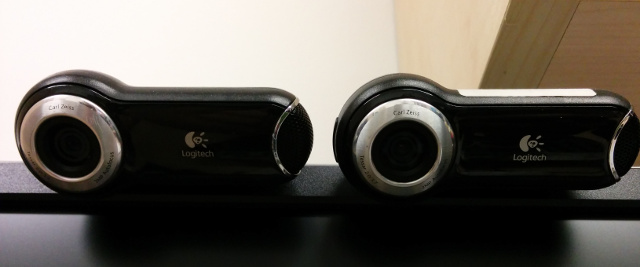
\includegraphics[width=300pt]{figures/scene1_camerapose.jpg}
\caption{Kamerák helyzete az első jelenetnél \label{fig:scene1_camerapose}}

\vspace{10pt}

% az első 53 frame droppolva
\begin{subfigure}[b]{.32\linewidth}
	\centering
	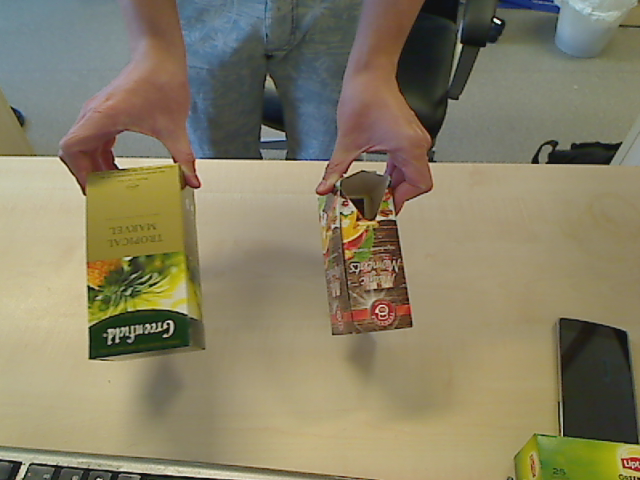
\includegraphics[width=135pt]{figures/left_93.png}
  \end{subfigure}
\begin{subfigure}[b]{.32\linewidth}
	\centering
	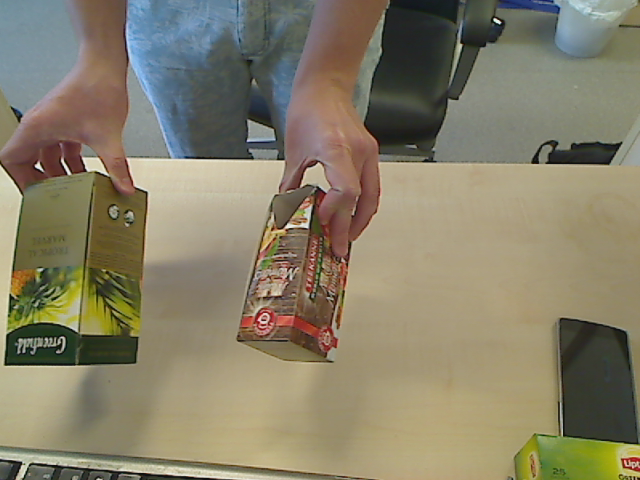
\includegraphics[width=135pt]{figures/left_153.png}
  \end{subfigure}
\begin{subfigure}[b]{.32\linewidth}
	\centering
	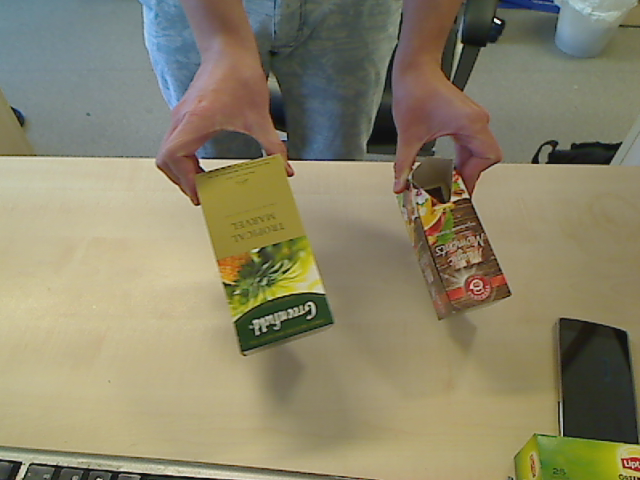
\includegraphics[width=135pt]{figures/left_223.png}
  \end{subfigure}\\\vspace{5pt}
\begin{subfigure}[b]{.32\linewidth}
	\centering
	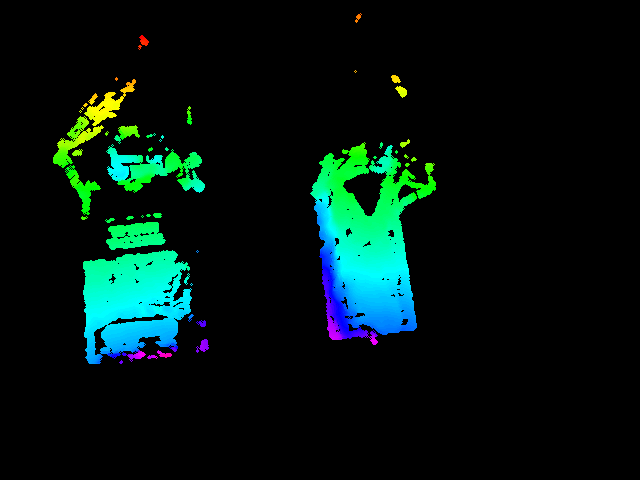
\includegraphics[width=135pt]{figures/vis_93.png}
  \end{subfigure}
\begin{subfigure}[b]{.32\linewidth}
	\centering
	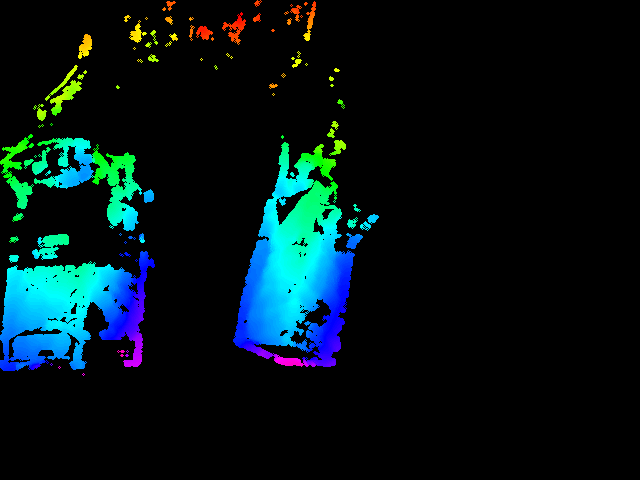
\includegraphics[width=135pt]{figures/vis_153.png}
  \end{subfigure}
\begin{subfigure}[b]{.32\linewidth}
	\centering
	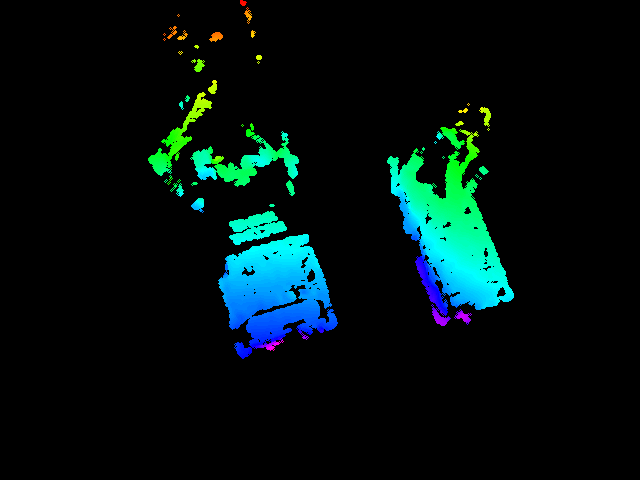
\includegraphics[width=135pt]{figures/vis_223.png}
  \end{subfigure}
\caption{A bal oldali kamera 3 képkockája (40., 100. és 170. képkocka) az első jelenetből, valamint a helyreállított képek a bal oldali kamera nézőpontjából \label{fig:scene1_frames}}

\vspace{10pt}

\begin{subfigure}[b]{.32\linewidth}
	\centering
	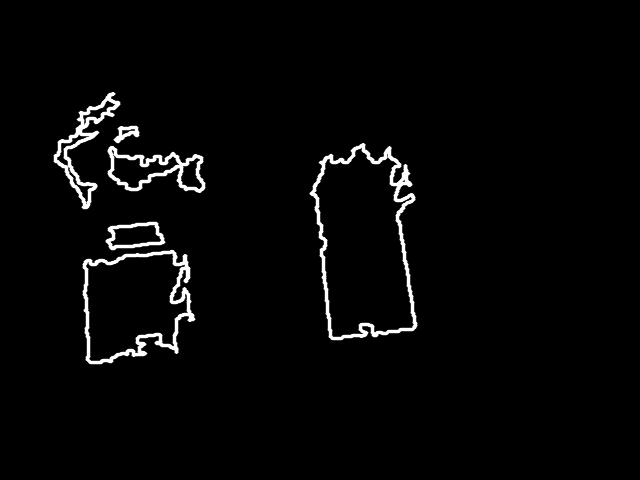
\includegraphics[width=135pt]{figures/contour_93.png}
  \end{subfigure}
\begin{subfigure}[b]{.32\linewidth}
	\centering
	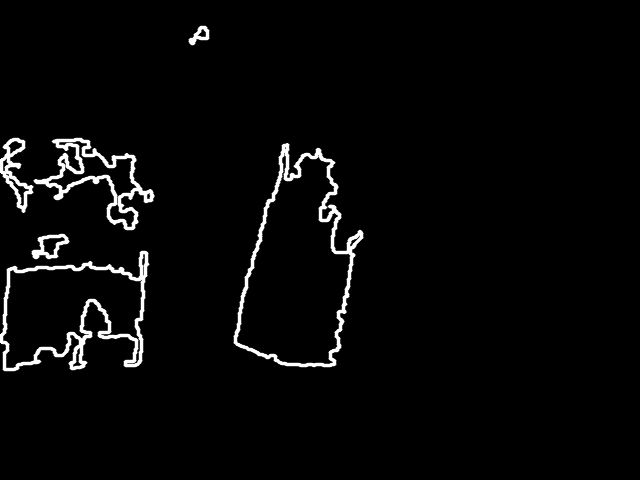
\includegraphics[width=135pt]{figures/contour_153.png}
  \end{subfigure}
\begin{subfigure}[b]{.32\linewidth}
	\centering
	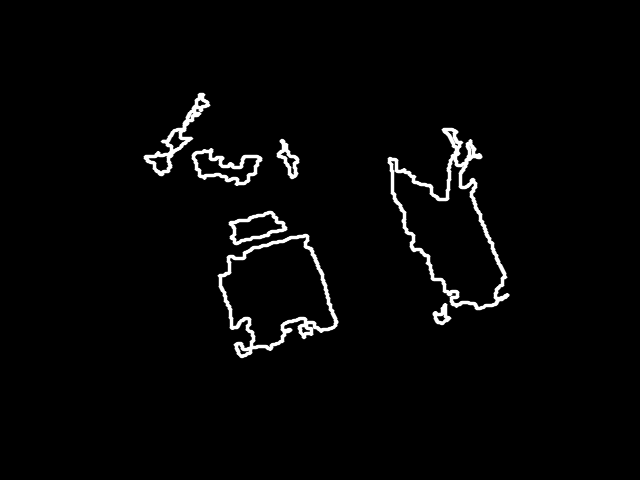
\includegraphics[width=135pt]{figures/contour_223.png}
  \end{subfigure}
\caption{A 40., 100. és 170. képkockák alapján számolt kontúrok a bal oldali kamera nézőpontjából \label{fig:scene1_contours}}

\end{figure}

% -------------------------------------------------------
\section{Második jelenet}
% -------------------------------------------------------

Második jelenet két olyan kamera által került rögzítésre, amelyek optikai tengelyei egy hegyes szöveg zártak be (lásd \ref{fig:scene2_camerapose}. ábra). Ebben az esetben is két teásdobozt mozgattam. A jelenet 360 képkockából állt (\textasciitilde 12 másodperc), melyből mindegyik $640\times 480$-as felbontású, színes kép. \Aref{fig:scene2_frames}. ábrán látható a bal oldali kamerák által rögzített 4 képkocka és ugyanezen nézőpontból vett helyreállítások vizualizációi.

\begin{figure}
\centering
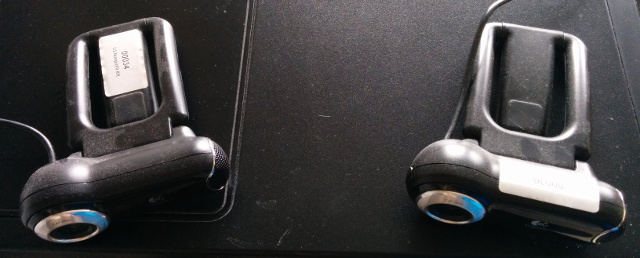
\includegraphics[width=280pt]{figures/scene2_camerapose.jpg}
\caption{Kamerák helyzete a második jelenetnél \label{fig:scene2_camerapose}}
\end{figure}

\begin{figure}[b!]
\centering
\begin{subfigure}[b]{.32\linewidth}
	\centering
	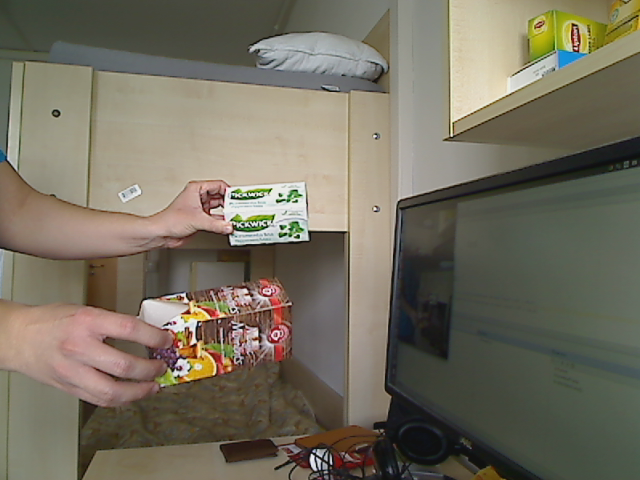
\includegraphics[width=135pt]{figures/scene2/left_45.png}
  \end{subfigure}
\begin{subfigure}[b]{.32\linewidth}
	\centering
	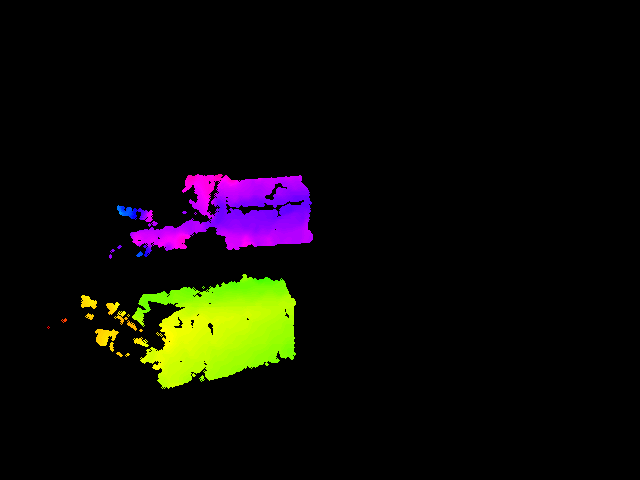
\includegraphics[width=135pt]{figures/scene2/vis_45.png}
  \end{subfigure}
\begin{subfigure}[b]{.32\linewidth}
	\centering
	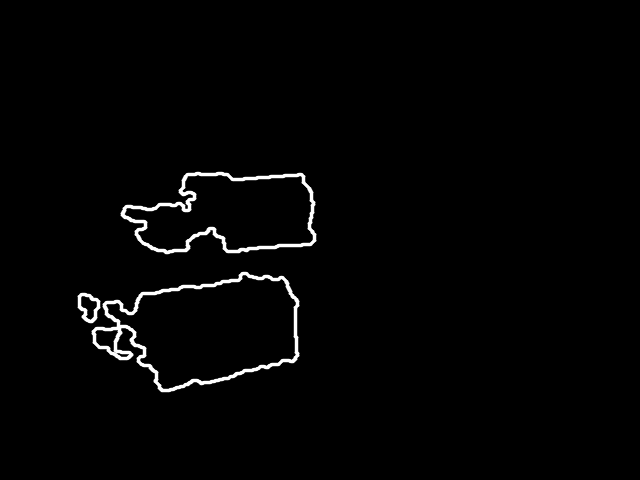
\includegraphics[width=135pt]{figures/scene2/ctr_45.png}
  \end{subfigure}\\\vspace{5pt}
  \begin{subfigure}[b]{.32\linewidth}
	\centering
	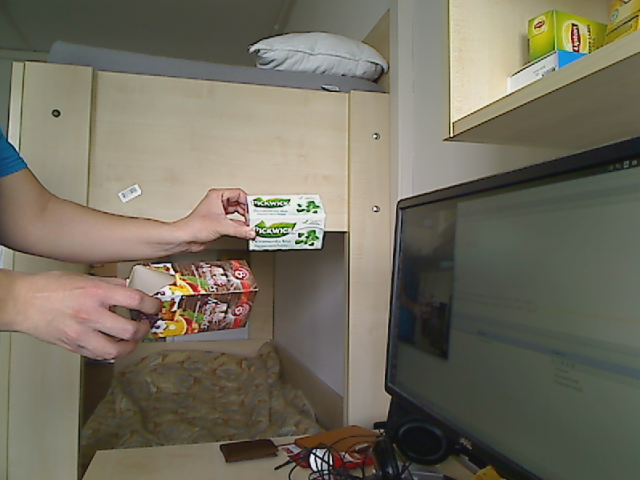
\includegraphics[width=135pt]{figures/scene2/left_130.png}
  \end{subfigure}
\begin{subfigure}[b]{.32\linewidth}
	\centering
	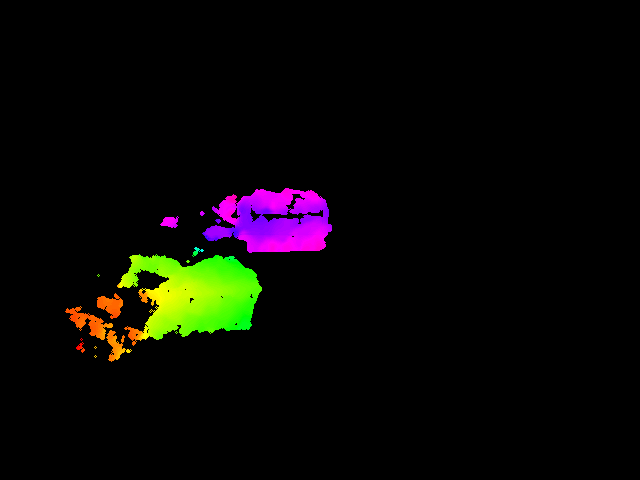
\includegraphics[width=135pt]{figures/scene2/vis_130.png}
  \end{subfigure}
\begin{subfigure}[b]{.32\linewidth}
	\centering
	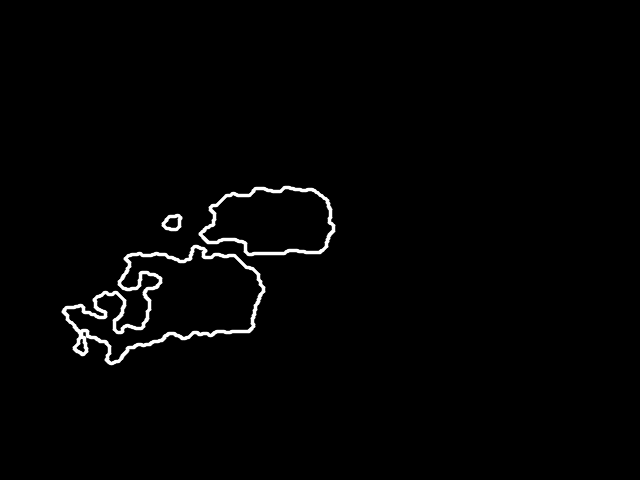
\includegraphics[width=135pt]{figures/scene2/ctr_130.png}
  \end{subfigure}\\\vspace{5pt}
  \begin{subfigure}[b]{.32\linewidth}
	\centering
	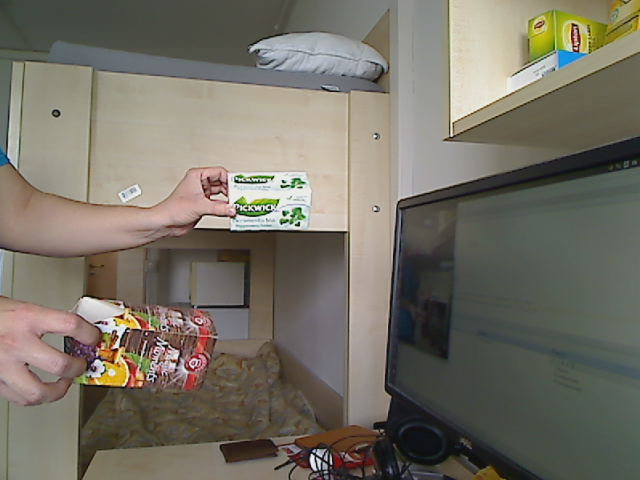
\includegraphics[width=135pt]{figures/scene2/left_215.png}
  \end{subfigure}
\begin{subfigure}[b]{.32\linewidth}
	\centering
	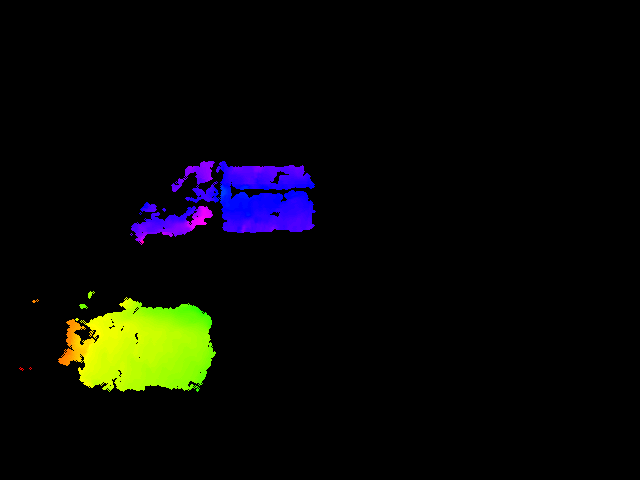
\includegraphics[width=135pt]{figures/scene2/vis_215.png}
  \end{subfigure}
\begin{subfigure}[b]{.32\linewidth}
	\centering
	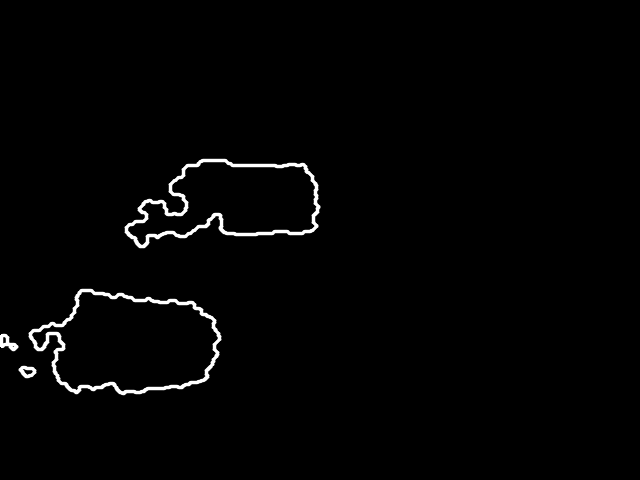
\includegraphics[width=135pt]{figures/scene2/ctr_215.png}
  \end{subfigure}\\\vspace{5pt}
  \begin{subfigure}[b]{.32\linewidth}
	\centering
	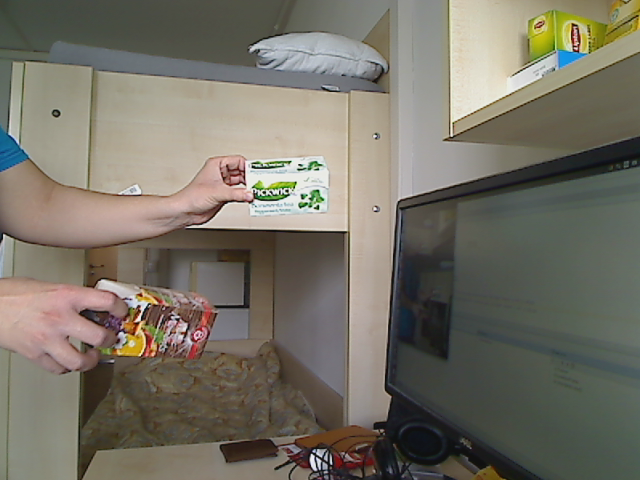
\includegraphics[width=135pt]{figures/scene2/left_339.png}
  \end{subfigure}
\begin{subfigure}[b]{.32\linewidth}
	\centering
	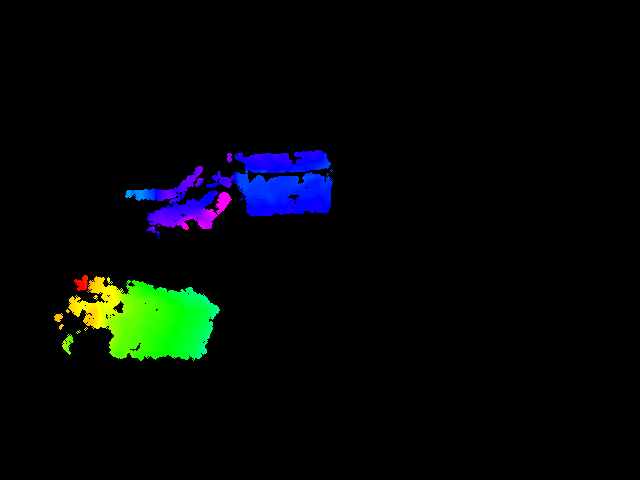
\includegraphics[width=135pt]{figures/scene2/vis_339.png}
  \end{subfigure}
\begin{subfigure}[b]{.32\linewidth}
	\centering
	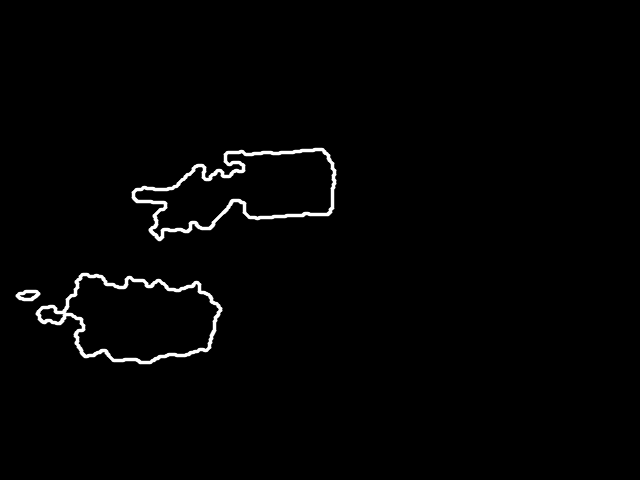
\includegraphics[width=135pt]{figures/scene2/ctr_339.png}
  \end{subfigure}
\caption{A második jelenethez tartozó 45., 130., 215. és 339. képkockák bal oldali képei és azok vizualizációi \label{fig:scene2_frames}}
\end{figure}

A képek jól mutatják, hogy elég sok pontot sikerült helyreállítani köszönhetően a jól textúrázott dobozoknak, a lassú mozgásnak és a megfelelő fényviszonyoknak. Az átlagos visszavetítési hiba ennél a jelenetnél 1,5 pixel lett.

\Aref{fig:scene2_close}. ábrán látható két olyan helyzet, amikor a két doboz a képeken nagyon közel volt egymáshoz. Az első esetben a hátul lévő dobozt szinte teljesen elveszítettük, míg a második esetben jól elkülönült térben az eredmény. Ekkor viszont a képen látható közelség miatt az előtér maszkok összemosódtak, így logikailag egy objektumként értelmeztük őket, amit a kontúrrajzon is megfigyelhetünk.

\begin{figure}
\centering
\begin{tikzpicture}[spy using outlines={white,chamfered rectangle, magnification=1.5, width=2cm, height=1.5cm, connect spies}]

\node (A) {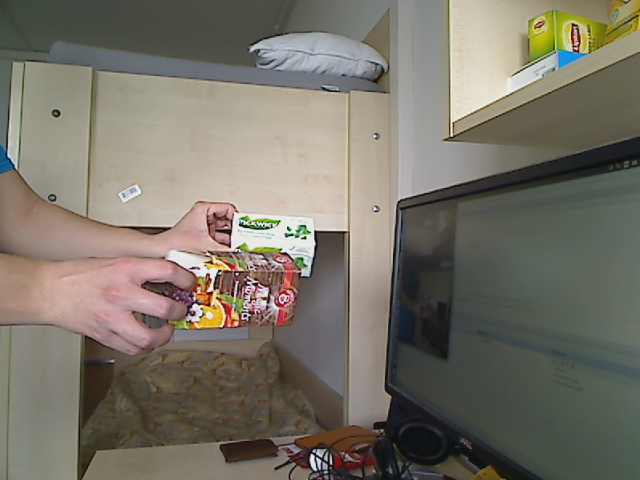
\includegraphics[width=135pt]{figures/scene2/left_182.png}};
%\spy on (-0.6,-0.2) in node [left] at (2.3,0.95);

\node (B) [right of=A,xshift=10.5em] {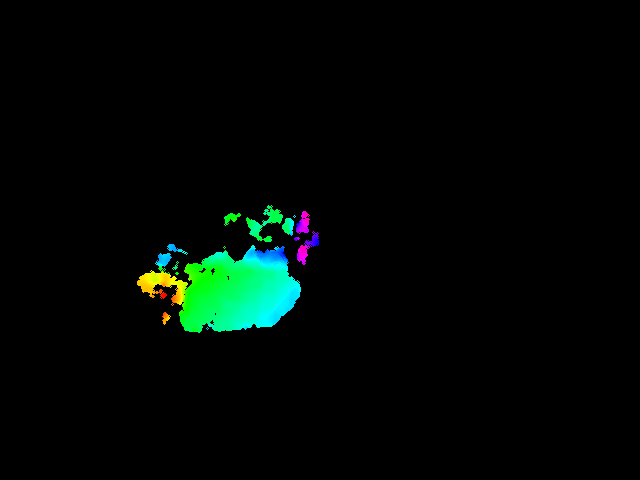
\includegraphics[width=135pt]{figures/scene2/vis_182.png}};

%\spy on ($(-0.6,-0.2)+(13.1em,0)$) in node [left] at ($(2.3,0.95)+(13.1em,0)$);

\node (C) [right of=B,xshift=10.5em] {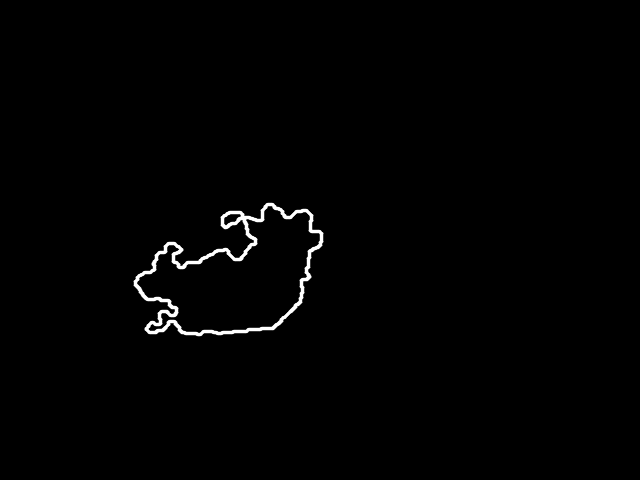
\includegraphics[width=135pt]{figures/scene2/ctr_182.png}};


\end{tikzpicture}\\\vspace{3pt}

\begin{tikzpicture}[spy using outlines={white,chamfered rectangle, magnification=1.5, width=2.1cm, height=1.7cm, connect spies}]

\node (A) {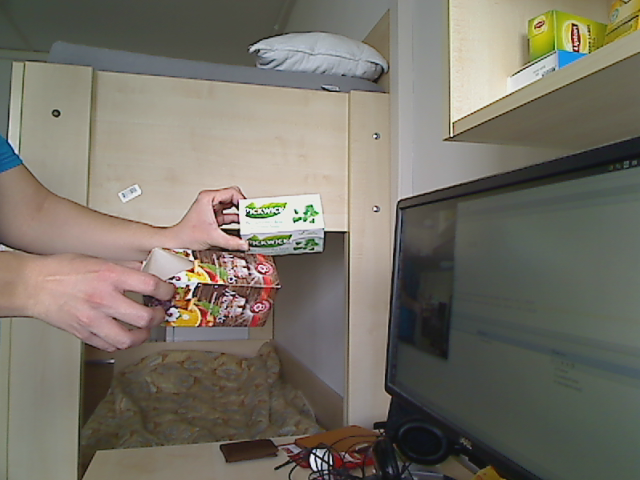
\includegraphics[width=135pt]{figures/scene2/left_192.png}};
%\spy on (-0.6,-0.17) in node [left] at (2.3,-0.95);

\node (B) [right of=A,xshift=10.5em] {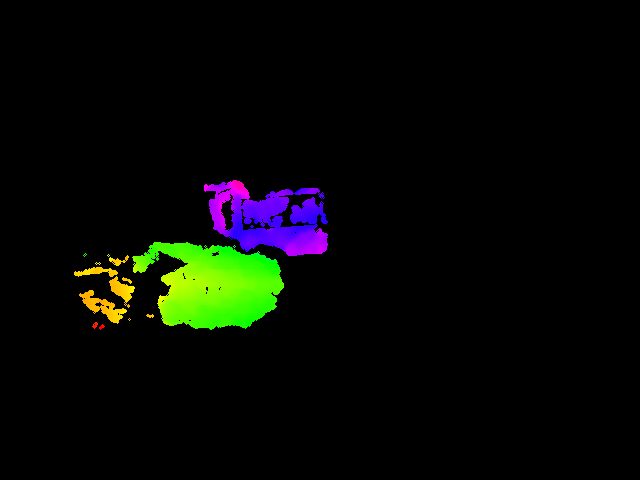
\includegraphics[width=135pt]{figures/scene2/vis_192.png}};

%\spy on ($(-0.6,-0.17)+(13.1em,0)$) in node [left] at ($(2.3,-0.95)+(13.1em,0)$);

\node (C) [right of=B,xshift=10.5em] {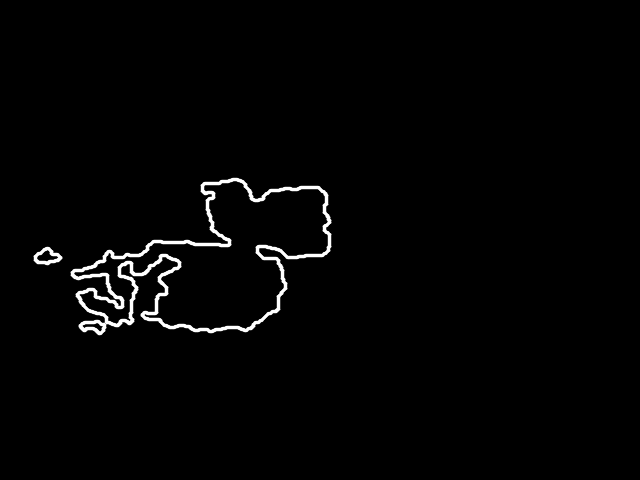
\includegraphics[width=135pt]{figures/scene2/ctr_192.png}};

\end{tikzpicture}

\caption{Amikor a két doboz közel van egymáshoz, kiemelve a részleteket \label{fig:scene2_close}}

\end{figure}

% -------------------------------------------------------
\section{Harmadik jelenet}
% -------------------------------------------------------

\begin{figure}[b]
\centering
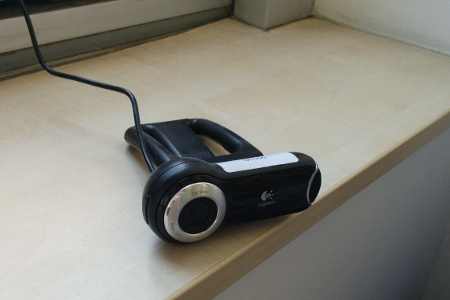
\includegraphics[width=180pt]{figures/scene3/scene3_cameraposeleft.jpg}\hspace{10pt}
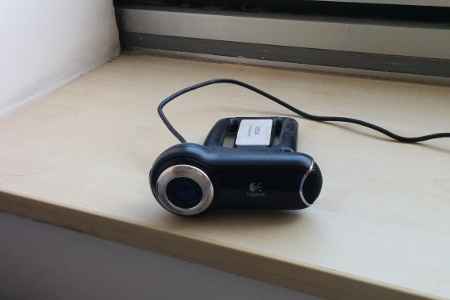
\includegraphics[width=180pt]{figures/scene3/scene3_cameraposeright.jpg}
\caption{A harmadik jelenetnél használt kamera elrendezés (bal és jobb kamera a párkány szélén) \label{fig:scene3_camerapose}}
\end{figure}

A harmadik jeleneten egy valós helyzethez igen közeli kamerabeállítást használtam (lásd \ref{fig:scene3_camerapose}. ábra), amikor egy megfigyelt terület két sarkába helyeztem a (megfigyelő) kamerákat. A jelenet során egy nagyobb textúrázott dobozt mozgattam és 500 képkockából álló videót készítettem (\textasciitilde 16,5 másodperc), melyből az eddigiekhez hasonlóan mindegyik $640\times 480$-as felbontású, színes kép volt. \Aref{fig:scene3_frames}. ábrán látható a két kamera által rögzített kép és a bal oldali kamera nézőpontjából helyreállított kép vizualizációja.

\begin{figure}
\centering
\begin{subfigure}[b]{.32\linewidth}
	\centering
	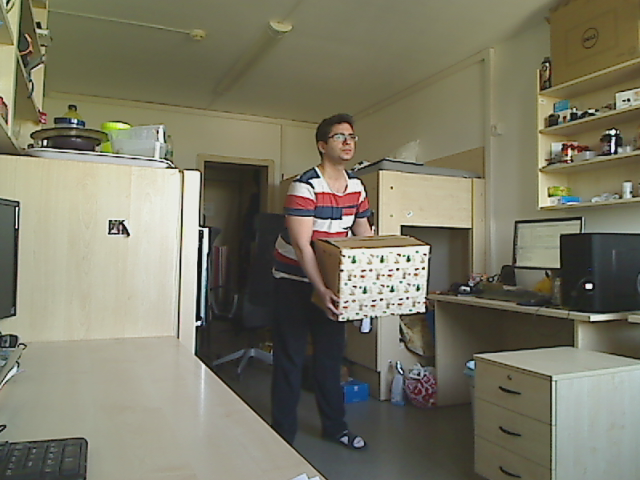
\includegraphics[width=135pt]{figures/scene3/left_152.png}
  \end{subfigure}
\begin{subfigure}[b]{.32\linewidth}
	\centering
	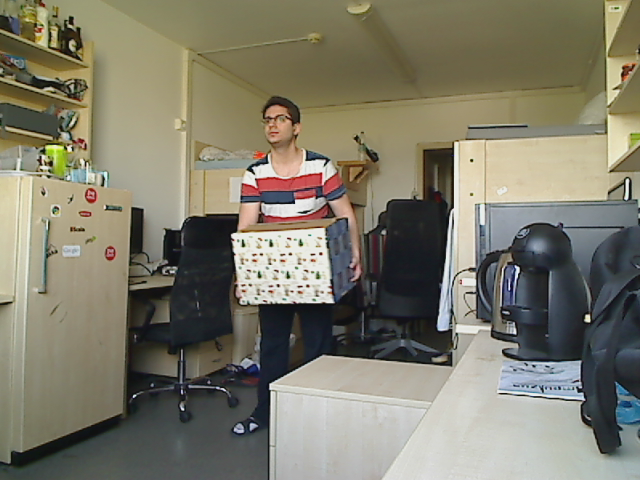
\includegraphics[width=135pt]{figures/scene3/right_152.png}
  \end{subfigure}
\begin{subfigure}[b]{.32\linewidth}
	\centering
	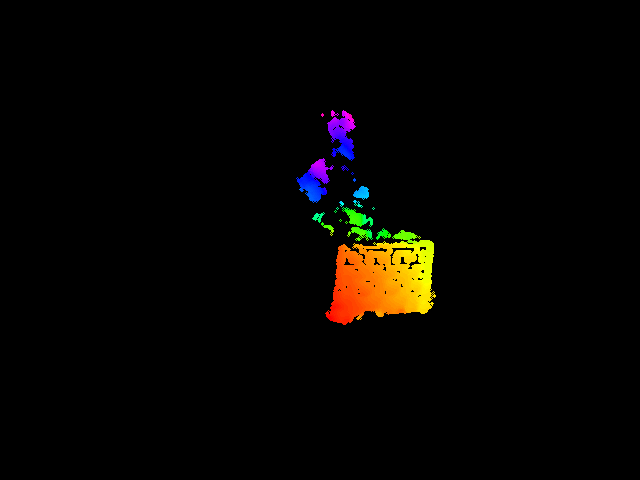
\includegraphics[width=135pt]{figures/scene3/vis_152.png}
  \end{subfigure}\\\vspace{5pt}
\begin{subfigure}[b]{.32\linewidth}
	\centering
	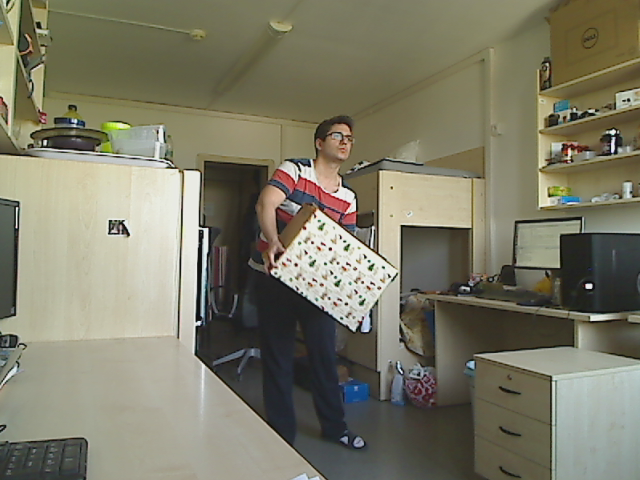
\includegraphics[width=135pt]{figures/scene3/left_196.png}
  \end{subfigure}
\begin{subfigure}[b]{.32\linewidth}
	\centering
	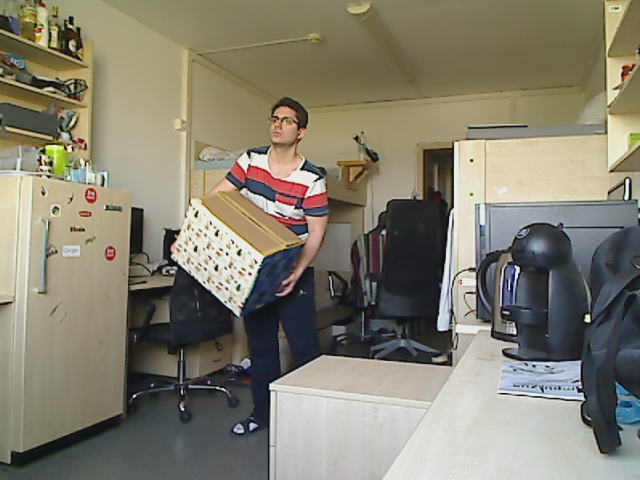
\includegraphics[width=135pt]{figures/scene3/right_196.png}
  \end{subfigure}
\begin{subfigure}[b]{.32\linewidth}
	\centering
	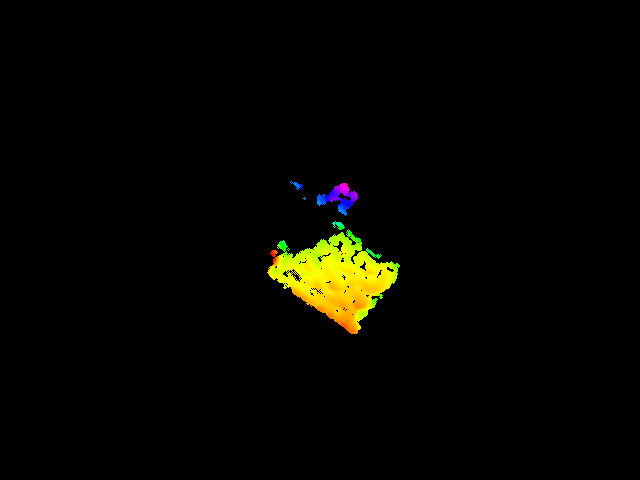
\includegraphics[width=135pt]{figures/scene3/vis_196.png}
  \end{subfigure}\\\vspace{5pt}
\begin{subfigure}[b]{.32\linewidth}
	\centering
	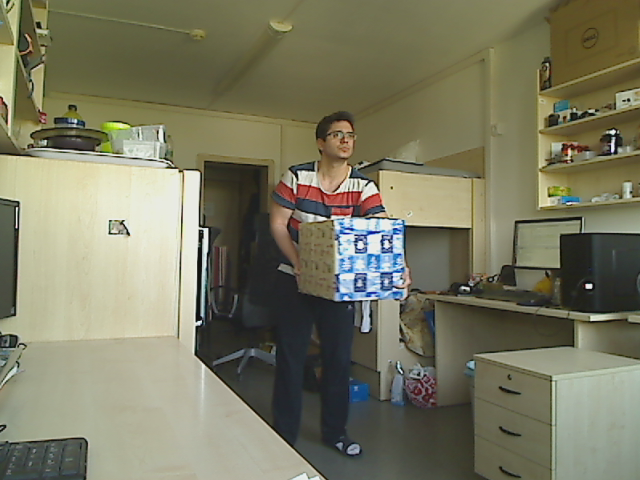
\includegraphics[width=135pt]{figures/scene3/left_376.png}
  \end{subfigure}
\begin{subfigure}[b]{.32\linewidth}
	\centering
	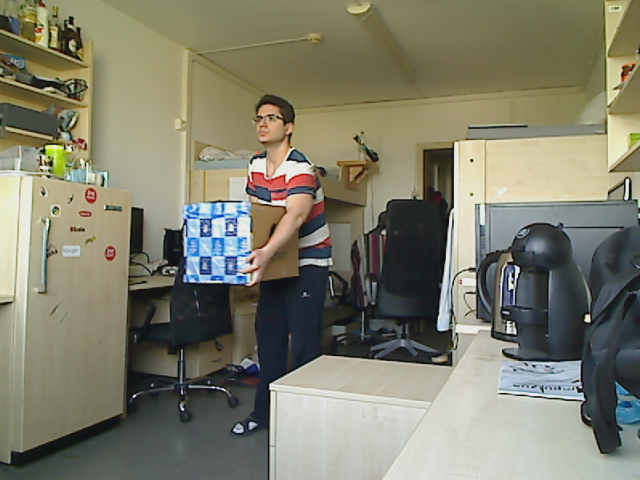
\includegraphics[width=135pt]{figures/scene3/right_376.png}
  \end{subfigure}
\begin{subfigure}[b]{.32\linewidth}
	\centering
	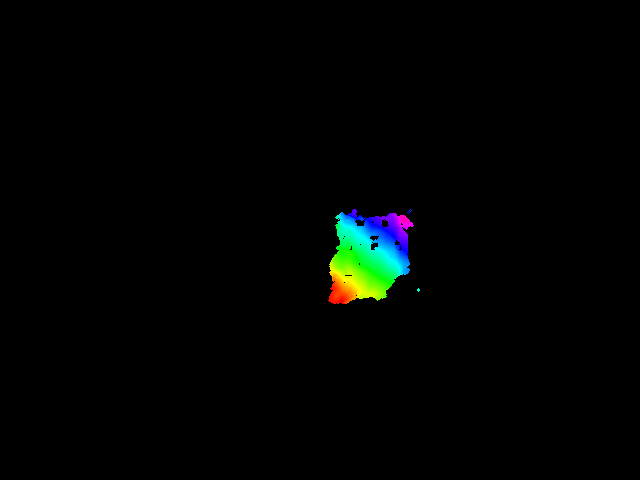
\includegraphics[width=135pt]{figures/scene3/vis_376.png}
  \end{subfigure}\\\vspace{5pt}
\begin{subfigure}[b]{.32\linewidth}
	\centering
	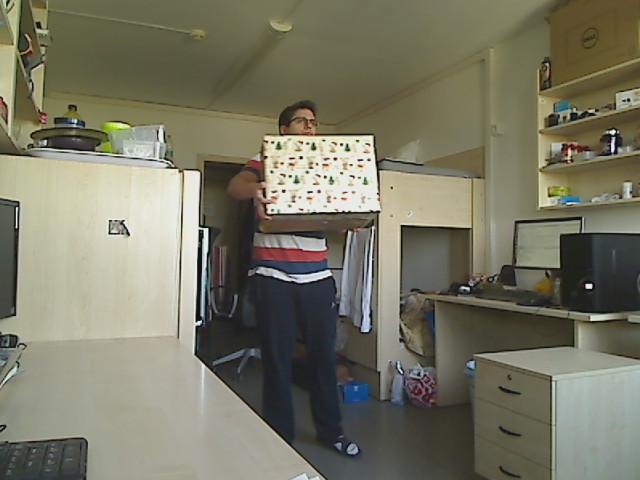
\includegraphics[width=135pt]{figures/scene3/left_468.png}
  \end{subfigure}
\begin{subfigure}[b]{.32\linewidth}
	\centering
	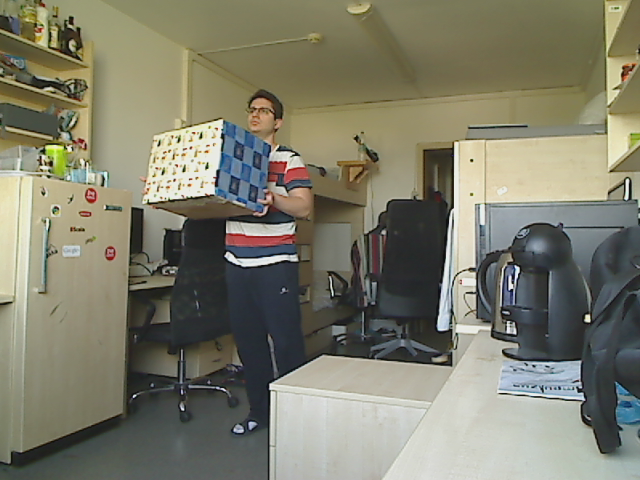
\includegraphics[width=135pt]{figures/scene3/right_468.png}
  \end{subfigure}
\begin{subfigure}[b]{.32\linewidth}
	\centering
	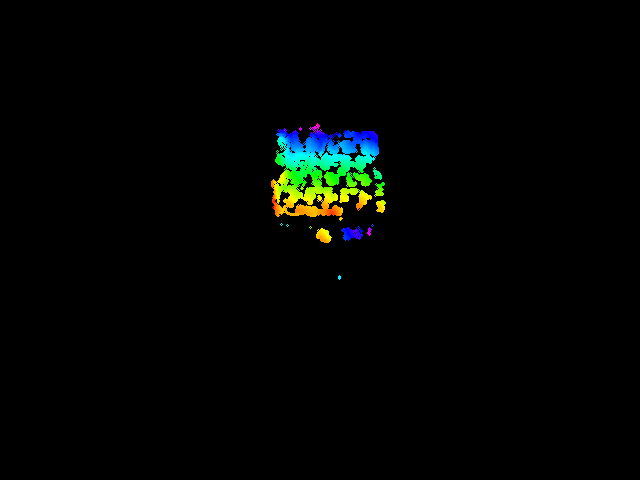
\includegraphics[width=135pt]{figures/scene3/vis_468.png}
  \end{subfigure}\\\vspace{5pt}
\caption{A második jelenethez tartozó 52., 96., 276. és 368. képkockák bal oldali képei és azok vizualizációi \label{fig:scene3_frames}}

\end{figure}

Ennél a jelenetnél is számos alkalommal (223 képkocka esetén) jól használható rekonstrukciókat kaptam, kivéve amikor megcsillant a napfény a fényes felületen, a mozgás túl hirtelen volt, így a kép elmosódott, vagy a doboz textúrázott oldala az egyik képen már túl hegyes szögben látszódott. Az átlagos visszavetítési hibára ezen képkockák esetén 2,56 pixel adódott.

% ---------------------
\section{Összefoglaló}
% ---------------------

Ebben a fejezetben három jelenet segítségével teszteltem a helyreállítást. Az eredmények alapján a tesztelést sikeresnek tekintettem. A tapasztalatok alapján, amennyiben eleget teszünk azon követelményeknek, miszerint az objektumok mozogjanak a képeken és a felületük textúrája ne legyen nagy felületeken egybefüggően homogén, akkor igen pontos és jól felismerhető rekonstrukciókat kapunk az elkészült megoldás segítségével. Az utolsó jelenet eredményei azt is igazolják, hogy egy szoba közepén játszódó eseménysorozat, annak két sarkából rögzített videófolyamok alapján a két nézőpont között szintén jó minőségben helyreállítható a dolgozatban leírt és megvalósított módszerrel.
